

\documentclass[aspectratio=169, 12pt]{beamer}

%%%%%%%%%%%%
% Packages %
%%%%%%%%%%%%

\usepackage{ctex}
\usepackage[english]{babel}
\usepackage{packages/sleek}
\usepackage{packages/tweaks}
\usepackage{calligra} % thanks pakeage
\usepackage{graphicx}

%%%%%%%%%%%%%%%%
% Bibliography %
%%%%%%%%%%%%%%%%

\addbibresource{./resources/bib/references.bib}

%%%%%%%%%%%%%%
% Title-page %
%%%%%%%%%%%%%%


\title{公共经济学}
\subtitle{Public Economics}
\author[LIU ShHUAI]{刘 {  } 帅}
\institute{山西师范大学 {  } 经济与管理学院}
\date{\today}
\titlelogo{./resources/pdf/logo.png}
\framelogo{./resources/pdf/logo.png}

%%%%%%%%%%%%
% Document %
%%%%%%%%%%%%

\begin{document}

\maketitle

\begin{frame}[plain]
    \frametitle{参考书目}
    公共部门经济学. 约瑟夫·E.斯蒂格利茨, 杰伊·K.罗森加德 著, 郭庆旺 译. 中国人民大学出版社. 2020年07月.
    \par
    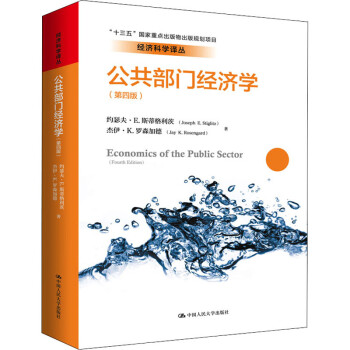
\includegraphics[height=5cm]{./resources/figure/pbook.png}
\end{frame}


\begin{frame}[standout]
    第二章\par
    \addtolength{\parskip}{.4em}
    绪{  }论
\end{frame}

\begin{frame}[plain]
    \frametitle{重点问题}
    \begin{itemize}
        \item \textbf{公共部门经济学研究的核心问题是什么?}
        \item \textbf{关于政府的经济作用,有哪些观点?这些观点有怎样的变化?这些变化的起因是什么?}
        \item \textbf{经济学家是如何研究公共部门经济学的?}
        \item \textbf{经济学家在政府应当采取的恰当政策上存在分歧的主要原因是什么?}
    \end{itemize}
\end{frame}

\begin{frame}[plain]
    % \begin{multicols}{1}
    %   \frametitle{Outline}
    %   \tableofcontents[hideallsubsections]
    % \end{multicols}
    \frametitle{Outline}
    \tableofcontents[hideallsubsections]
    % \tableofcontents[currentsection]
  \end{frame}

\section{一、公共经济学的源起}

\begin{frame}[plain]
    \frametitle{公共经济学的产生}
    公共经济学是从研究公共产品如何提供的问题作为发端而逐渐发展形成的,基本形成于20世纪五六十年代。
    \par
    其起源的标志是美国经济学家萨缪尔森1954年《公共支出的纯理论》一文的发表。
    \par
    1959年,美国经济学家马斯格雷夫的著作《公共财政学理论:公共经济研究》出版,首次引入公共经济的概念,标志着公共经济学作为一门学科正式诞生。
    \par
    斯蒂格利茨、阿特金森等为代表的经济学家开始公共经济学的研究。
    \par
    1966年,阿特金森主持公共经济学学会成立及会刊创立。
    \par
    1972年,布坎南《公共选择理论》一书出版。
\end{frame}

\section{二、公共经济学的定义及研究对象}

\begin{frame}[plain]
    \frametitle{公共经济学的定义}
    公共经济学就是经济学中专门研究\textbf{公共部门经济行为}特殊规律的分支学科,
    是论述各级政府和其他公共部门的存在意义和行为,回答他们必须\textbf{做什么以及应该怎样做}的学问。
    \par
    根据最一般的的定义,公共经济学是对\textbf{经济效率、分配和政府经济政策}的研究
\end{frame}

\begin{frame}[plain]
    \frametitle{公共部门的活动}
    公共部门的活动以各种方式影响着我们的生活。
    \begin{figure}
        \centering
        \begin{minipage}[t]{0.5\linewidth}
            \centering
            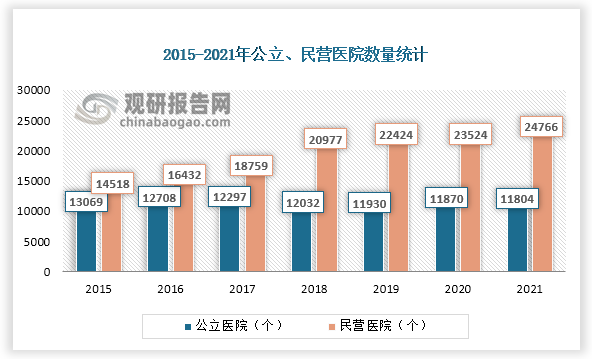
\includegraphics[width=1.0\textwidth]{./resources/figure/medical1.png}
        \end{minipage}%
        \begin{minipage}[t]{0.5\linewidth}
            \centering
            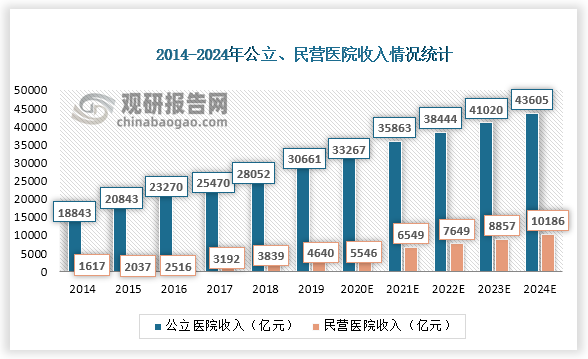
\includegraphics[width=1.0\textwidth]{./resources/figure/medical2.png}
        \end{minipage}
    \end{figure}
\end{frame}

\begin{frame}[plain]
    \frametitle{公共部门的活动}
    \begin{figure}
        \centering
        \begin{minipage}[t]{0.5\linewidth}
            \centering
            
\includegraphics[width=1.0\textwidth]{./resources/figure/insurence.jpeg}
        \end{minipage}%
        \begin{minipage}[t]{0.5\linewidth}
            \centering
            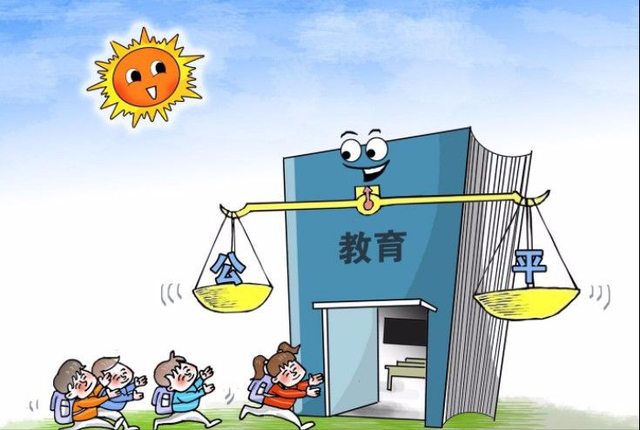
\includegraphics[width=1.0\textwidth]{./resources/figure/education.png}
        \end{minipage}
    \end{figure}
\end{frame}

\begin{frame}[plain]
    \frametitle{公共部门的活动}
    \begin{figure}
        \centering
        \begin{minipage}[t]{0.5\linewidth}
            \centering
            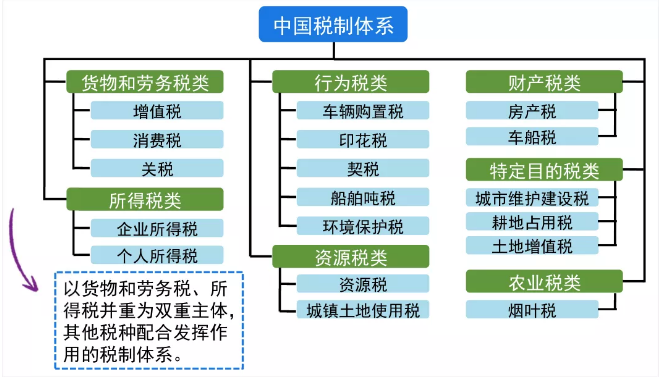
\includegraphics[width=1.0\textwidth]{./resources/figure/tax.png}
        \end{minipage}%
        \begin{minipage}[t]{0.5\linewidth}
            \centering
            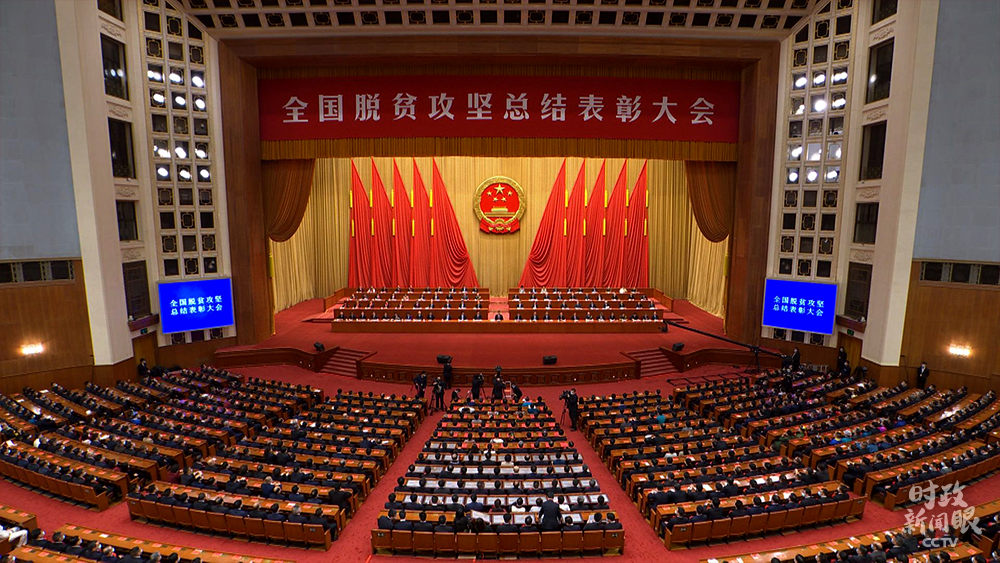
\includegraphics[width=1.0\textwidth]{./resources/figure/reversepoor.jpg}
        \end{minipage}
    \end{figure}
\end{frame}

\begin{frame}[plain]
    \frametitle{公共部门的活动}
    \begin{figure}
        \centering
        \begin{minipage}[t]{0.5\linewidth}
            \centering
            
\includegraphics[width=1.0\textwidth]{./resources/figure/ct.png}
        \end{minipage}%
        \begin{minipage}[t]{0.5\linewidth}
            \centering
            
\includegraphics[width=1.0\textwidth]{./resources/figure/wealth.jpg}
        \end{minipage}
    \end{figure}
\end{frame}

\begin{frame}[plain]
    \frametitle{公共部门的活动}
    \begin{figure}
        \centering
        \begin{minipage}[t]{0.5\linewidth}
            \centering
            
\includegraphics[width=1.0\textwidth]{./resources/figure/lawn.jpg}
        \end{minipage}%
        \begin{minipage}[t]{0.5\linewidth}
            \centering
            
\includegraphics[width=1.0\textwidth]{./resources/figure/co.jpg}
        \end{minipage}
    \end{figure}
\end{frame}

\begin{frame}[plain]
    \frametitle{公共经济学的研究对象}
    \textbf{什么是公共部门?} \par
    \addtolength{\parskip}{.8em}
    公共部门与私人部门相对应,被国家授予公共权力,
    并以社会的公共利益为组织目标,管理各项社会公共事务,
    向全体社会成员提供法定服务的政府和非政府组织。\par
    \addtolength{\parskip}{.8em}
    公共部门大致可以分为\textbf{政府、公共企业和非盈利组织}三类。
\end{frame}

\begin{frame}[plain]
    \frametitle{公共经济学的研究对象}
    \begin{block}{政府}
        \textbf{中央政府}:管理国家事务的国家机构总称。
        世界各国的中央政府有不同的名称,
        如国务院、政务院、国务委员会、部长会议、内阁等。
        \par
        \textbf{地方政府}:管理一个国家行政区事务的政府组织。
        地方政府的权力是中央政府依据宪法赋予的。
    \end{block}
    \begin{block}{公共企业}
        政府出于向社会公众提供必不可少的公共产品和服务、
        增进社会公正、调节和平衡宏观经济发展等目的建立和经营的企业。
        如:\textbf{环卫、自来水、公共交通…… }。
    \end{block}
    \begin{block}{非盈利组织}
        不以营利为目的,支持或处理公众关注的议题或事件的组织。
        如艺术、慈善、政治、宗教、学术、环保等团体。
        \textbf{世界卫生组织、世界气象组织}。
    \end{block}
\end{frame}

\section{三、政府的经济作用}

\begin{frame}[plain]
    \frametitle{公共经济学研究的制度背景}
    公共经济学研究的制度背景总是设为\textbf{混合经济(minxed economy)},
    即一方面尊重个体决策,另一方面政府又试图通过其实施的政策影响个体决策。
    \par
    关注混合经济使我们的分析能够应用于多数发达和发展中经济体,
    也使我们能够研究政府如何行事及政府应该如何行事。
\end{frame}

\begin{frame}[plain]
    \frametitle{关于政府作用的不同观点}
    \textbf{市场派}:信奉“看不见的手”,自由放任思想,
    政府对私人部门要敬而远之,别总想管控私人企业,
    无约束的竞争会使社会利益最大化。
    \par
    \textbf{政府派}:国家要在控制生产资料上发挥更大作用,积极的干预生产、分配。
    \par
    \textbf{现在普遍认为,市场和私人企业是经济成功的核心,但政府作为市场的补充同样举足轻重。}
    \begin{figure}[htbp]
        \centering
        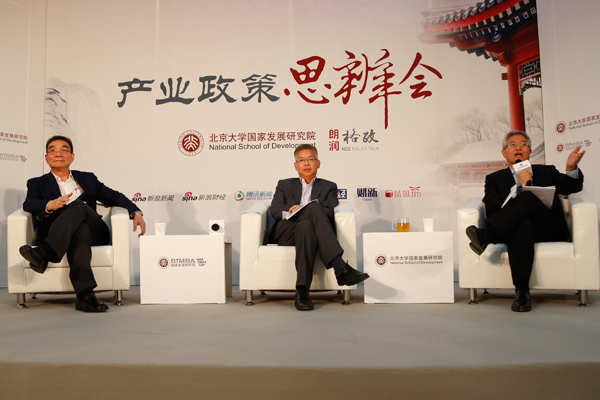
\includegraphics[width=0.57\textwidth]{./resources/figure/bate.jpg}
    \end{figure}
\end{frame}


\begin{frame}[plain]
    \frametitle{政府行为的动因}
    \textbf{市场失灵},市场在某一重要环节失效,政府就应该矫正这种市场失灵。
    1929年美国大萧条,失业率高达25\%,GDP下降三分之一。银行倒闭、股市崩盘,
    出现大量违约,美国经济无能为力。\par
    为了应对大萧条,美国联邦政府努力稳定经济,并且通过立缓解许多问题,包括
    失业保险、社会保障、联邦存款保险、联邦农产品价格支持计划,这些统称新政。
    \par
    还有另外两种市场失灵:一是\textbf{经济过度波动},2008年金融危机以及自1980年放松管制时代以来
    世界各地发生百余次危机就是证明。二是\textbf{不平等程度加剧},经济机会减少。
\end{frame}

\begin{frame}[plain]
    \frametitle{实现公共部门与私人部门间的平衡}
    市场常常失灵,市场解决不了的问题有很多。只有在相当严格的假设条件下,市场才完全有效。
    \par
    认识到市场的局限性,政府就应该只讲精力用于市场失灵最显著且有证据表明政府
    干预可以发挥重要作用的领域。
    \par
    但由于人们对市场失灵的严重程度和对政府矫正市场失灵的有效程度的看法不一,不同的观点由此产生。
    \begin{enumerate}
        \item 混合经济中,公共部门和私人部门都发挥重要作用。
        \item 政府所起的作用以及关于政府应该起怎样的作用的观点,因时而异。
        \item 政府从事特定活动的重要动因是现实存在的或所认识到的市场失灵。
        \item 除了市场失灵,人们越来越意识到政府也有局限性——“政府失灵”。
    \end{enumerate}
\end{frame}

\section{四、公共经济学研究思维和方法}

\begin{frame}[plain]
    \frametitle{公共部门经济学家的思维}
    像所有经济学家一样,公共部门经济学家也关注以下四个核心问题:
    \begin{enumerate}
        \item \textbf{生产什么?}
        \item \textbf{如何生产?}
        \item \textbf{为谁生产?}
        \item \textbf{如何决策?}
    \end{enumerate}
\end{frame}

\begin{frame}[plain]
    \frametitle{公共部门经济学家的思维}
    \begin{itemize}
        \item \textbf{生产什么?}我们要用多少资源生产公共产品,如国防和公路?
        我们要用多少资源生产私人产品,如汽车、电视机和电子游戏等?
    \end{itemize}
    \begin{minipage}{0.3\textwidth}
        我们通常用生产可能性曲线描述这种选择,描述了两类物品在技术和资源
    既定的情况下可以有效生产出来的各种数量。
    \end{minipage}
    \begin{minipage}{0.65\textwidth}  
        \centering
        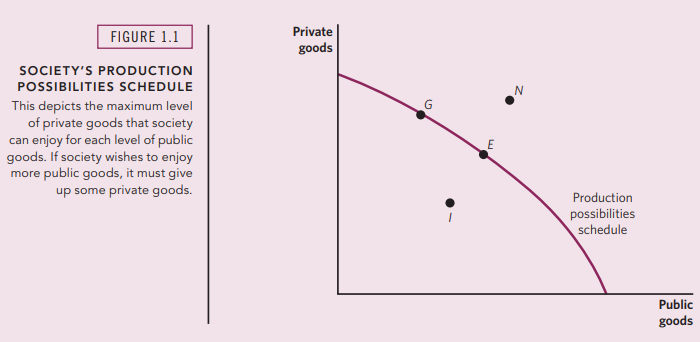
\includegraphics[width=1.0\textwidth]{./resources/figure/production.png}
    \end{minipage}
\end{frame}

\begin{frame}[plain]
    \frametitle{公共部门经济学家的思维}
    \begin{itemize}
        \item \textbf{如何生产?}
    \end{itemize}
    这一问题包含以下决策:是有私人生产,还是由公共生产?
    是多用资本、少用劳动,还是相反?是否采用节能技术?
    \par
    诸如此类的问题比比皆是。政府政策也会影响企业如何生产:
    环境保护法限制企业污染;去哦也必须为雇员缴纳五险一金,
    可能导致劳动更加昂贵,从而阻碍企业采用需要更多劳动的技术。
\end{frame}

\begin{frame}[plain]
    \frametitle{公共部门经济学家的思维}
    \begin{itemize}
        \item \textbf{为谁生产?(分配问题)}
    \end{itemize}
    政府有关税收或福利计划的决策会影响不同的人的支出。
    同样的,政府必须决定生产什么公共产品。有些群体会从
    一种公共产品中受益,而有些群体则会从另一种公共产品中受益。
    比如区域性的发展战略规划,西部大开发,中部崛起,东北振兴等。
\end{frame}

\begin{frame}[plain]
    \frametitle{公共部门经济学家的思维}
    \begin{itemize}
        \item \textbf{如何决策?}
    \end{itemize}
    在公共部门,选择是集体做出的。集体选择是社会必须一起做出的选择,
    比如关于法律体系、军事设施规模、其他公共产品支出等选择。
    \par
    公共部门经济学的目标之一就是研究民主社会中集体选择(有时称为社会选择)
    如何做出。集体选择相当复杂,因为人们常常不能就何为可取达成一致。
    \par
    认识到这种意见分歧本身很重要。我们要提妨诸如此类的言辞:“这是为了公共利益”
    或“我们关心社会利益”。不同的政策可能给不同的人带来好处,我们要谨慎确定谁将
    从既定政策中受益,谁将受损。
\end{frame}

\begin{frame}[plain]
    \frametitle{公共部门分析} 
    \begin{enumerate}
        \item \textbf{描述政府所为}:了解公共部门从事什么活动,这些活动是如何组织的。
        \item \textbf{分析政府行为的后果}:理解并尽可能预测这些政府活动的全部后果。政府政策的后果通常极其复杂,难以转却预测,即使在政策实施之后,人们也常常对其效果议论纷纷。
        \item \textbf{政策评估}:首先了解政策目标,然后确定在多大程度上符合政策目标和标准。
        \item \textbf{解释政治程序}:游戏规则是什么,什么决定游戏规则的选择。
    \end{enumerate}
\end{frame}

\begin{frame}[plain]
    \frametitle{公共部门经济学研究方法} 
    使用\textbf{经济模型}分析各种政策的效果。
    \begin{block}{实证经济学}
        关注“是”什么,描述经济的运行情况,当经济学家们描述经济、
        构建模型预测经济将如何变化或不同政策的影响时,所做的是
        实证经济学。
    \end{block}
    \begin{block}{规范经济学}
        解决“应该是”什么,对各种行动措施的可取性做出判断,当经济学家试图评价
        不同政策、权衡各种受益和成本时,他们所做的是规范经济学。
    \end{block}
\end{frame}

\begin{frame}[plain]
    \frametitle{公共部门经济学研究方法} 
    “我们应该减少贫困来降低人们的营养不良和促进经济增长。”
    区分出这句话中的的实证分析部分和规范分析部分。
    \par
    “维持一定的失业人口在经济上是有效率的。”请问这句话是实证判断还是规范判断?
    \par
    “高收入者应该承担更高的税率,因为他们的劳动供给无弹性。从高收入者中获得的
    税收收入可用于帮助低收入者。”区分这句判断中的实证判断部分和规范判断部分。
\end{frame}

\section{五、经济学家的意见分歧}

\begin{frame}[plain]
    \frametitle{经济学家的意见分歧} 
    \begin{block}{对有关经济行为的意见分歧}
        最优模型(个体如何做出反应)和数量大小(反应程度多少)
    \end{block}
    \begin{block}{有关价值判断的意见分歧}
        任何政策即产生可取的结果,也产生某些不良的后果。人们会以不同的
        方式权衡这些结果,取决于不同人的价值观。
    \end{block}
\end{frame}

% ---------------------------------------------------------------------------
\begin{frame}[standout]
    \begin{center}
        {\Huge\calligra Thanks!}
      \end{center}
\end{frame}
% ---------------------------------------------------------------------------

\end{document}
